\section{Entanglement and its applications}

A n-qubit state $\statepsi$ $(n \geq 2)$ is called \underline{entangled} if it cannnot be written 
as a tensor product of single-qubit states; i.e

\begin{equation}
    \statepsi \neq \ket{\psi_{n-1}} \otimes \cdots \otimes \ket{\psi_0}
\end{equation}

Example: Bell states, also denoted EPR states (Einstein, Podolsky, Rosen):

\begin{align*}
    \ket{\beta_{00}} &= \frac{1}{\sqrt{2}} (\ket{00} + \ket{11}) \\
    \ket{\beta_{01}} &= \frac{1}{\sqrt{2}} (\ket{01} + \ket{10}) \\
    \ket{\beta_{10}} &= \frac{1}{\sqrt{2}} (\ket{00} - \ket{11}) \\
    \ket{\beta_{11}} &= \frac{1}{\sqrt{2}} (\ket{01} - \ket{10}) \\
\end{align*}

\begin{figure}[H]
    \centering
    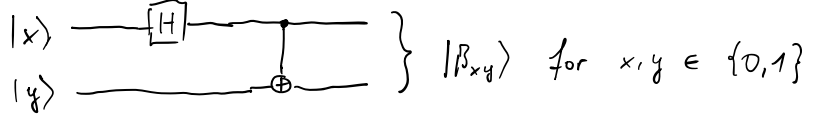
\includegraphics[scale=0.5]{chapters/res/circuit-bell-states.png}
    \caption{Quantum circuit to create Bell states}
\end{figure}


\subsection{Quantum teleportation}

Scenario: two (experimental physicists) Alice and Bob, are far away from each other

\begin{figure}[H]
    \centering
    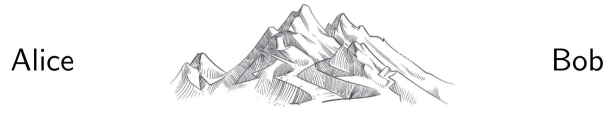
\includegraphics[scale=0.5]{chapters/res/alice-bob-mountains.png}
\end{figure}

When visiting each other a long time ago, they generated the EPR pair $\ket{\beta_{00}}$ each keeping on qubit of the pair.
Alice's task is to send another (unkown) qubit $\statepsi$ to Bob.
Note: Measurement is not an option.

\begin{figure}[H]
    \centering
    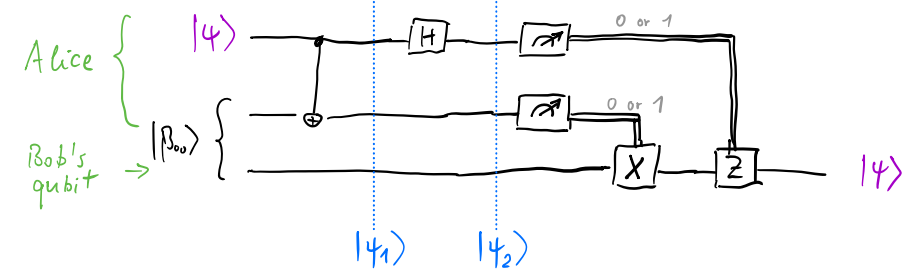
\includegraphics[scale=0.42]{chapters/res/circuit-teleporting-psi.png}
    \caption{Quantum circuit for teleporting $\statepsi$}
\end{figure}

Input:

\begin{equation*}
    \statepsi \ket{\beta_{00}} = (\alpha \ket{0} + \beta \ket{1}) \otimes \ket{\beta_{00}} 
        = \frac{1}{\sqrt{2}} \left[\alpha \ket{0} (\ket{00} + \ket{11}) + \beta \underbrace{\ket{1} (\ket{00} + \ket{11}}_{\text{CNOT}})\right]
\end{equation*}

after CNOT:
\begin{equation*}
    \ket{\psi_1} = \frac{1}{\sqrt{2}} 
        \left[\alpha \ket{0} (\ket{00} + \ket{11}) + \beta \ket{1} (\ket{{\color{red}1}0} + \ket{{\color{red}0}1})\right]
\end{equation*}

after Hadamard:
\begin{align*}
    \ket{\psi_2} &= \frac{1}{2} 
        [\alpha (\ket{0} + \ket{1})  \cdot
            (\ket{00} + \ket{11})]
        + \beta (\ket{0} - \ket{1}) \cdot 
            ((\ket{10} + \ket{01})) \\
    %
    &= \frac{1}{2} (\alpha \ket{000} + \alpha \ket{011} \alpha \ket{100} + \alpha \ket{111})
        + \beta \ket{010} + \beta \ket{001} - \beta \ket{110} - \beta \ket{101}) \\
    %
    &= \frac{1}{2} (\alpha \ket{000} + \alpha \ket{011} + \alpha \ket{100} + \alpha \ket{111}) + 
        \beta \ket{010} + \beta \ket{001} - \beta \ket{110} - \beta \ket{101} \\
    %
    &= \frac{1}{2} (\ket{00} (\alpha \ket{0} + \beta \ket{1}) + \ket{01} (\alpha \ket{1} + \beta \ket{0}))
        + \ket{10} (\alpha \ket{0} - \beta \ket{1}) + \ket{11} (\alpha \ket{1} - \beta \ket{0}))
\end{align*}

Now Alice measures her qubits w.r.t computational basis, e.g. projective measurement with 

\begin{align*}
    P_1 &= \ket{00} \bra{00} \otimes I, \quad P_2 = \ket{01} \bra{10} \otimes I \\ 
    P_3 &= \ket{10} \bra{10} \otimes I, \quad P_2 = \ket{11} \bra{11} \otimes I \\ 
\end{align*}

If Alice measures $\ket{00}$, then $\ket{\psi_2}$ will collapse to 
\begin{equation*}
    \ket{00} (\alpha \ket{0} + \beta \ket{1}) = \ket{00} \underbrace{\statepsi}_{\text{Qubit at Bob's place}}
\end{equation*}

similarly:

\begin{align*}
    00 &\mapsto \alpha \ket{0} + \beta \ket{1} \\
    01 &\mapsto \alpha \ket{1} + \beta \ket{0} \\
    10 &\mapsto \alpha \ket{0} - \beta \ket{1} \\
    11 &\mapsto \alpha \ket{1} - \beta \ket{0} 
\end{align*}

Alice transmits her measurement result to Bob (classical information), Bob then applies
Pauli-X and / or Pauli-Z to recover $\statepsi$. Even though wavefunction collapse is 
instantaneous, no faster-than-light transfer possible due to required classical communication.

\subsection{EPR and the Bell inequality}
EPR: Einstein, Podolsky, Rosen
EPR paper: \textit{"Can quantum mechanical description of physical relatiy be considered complete?"} (1935) \\
%
The another argue that quantum mechanics is incomplete since it lacks certain "elements of reality" 
(property can be predicted with certainity).

Scenario: Alice and Bob are far from each other, but share the entangled two-qubit "spin-singlet" state
\begin{equation*}
    \ket{\beta_{11}} = \frac{1}{\sqrt{2}} (\ket{01} - \ket{10})
\end{equation*}

Alice and Bob measure the observable $\vec{v} \circ  \vec{\sigma} = v_1 X + v_2 Y + v_3 Z$ 
(with $v \in \mathbb{R}^3, \norm{\vec{v}} = 1$) on their respective qubit.
(Recall $\vec{v} \circ \vec{\sigma}$ is Hermitian and unitary, and has eigenvalues $\pm 1$)

Alice performs her measurement immediately before Bob.
Example:
\begin{itemize}
    \item $\vec{v} = (0, 0, 1)^T$, observable $Z = 1 \cdot \ket{0} \bra{0} + (-1) \cdot \ket{1} \bra{1}$
        (standard measurement) \\
        if alice measures eigenvalue
        \begin{align*}
            1: &\quad \text{wavefunction collapses to } \ket{01} \\
            0: &\quad \text{wavefunction collapses to } \ket{10}
        \end{align*}
        $\leadsto$ Bob will always obtain the opposite measurement result.
    
    \item $\vec{v} = (1, 0, 0)^T$, observable: $X$, eigenstates 
    $\ket{\pm} = \frac{1}{\sqrt{2}}(\ket{0} + \ket{1})$, corresponding eigenvalues
    $\pm 1$ (measurement w.r.t $\{\ket{+}, \ket{-}\}$ basis) \\
    Can represent the wavefunction
    \begin{equation}
        \ket{\beta_{11}} = \frac{-1}{\sqrt{2}} (\ket{+-} - \ket{-+})
    \end{equation}
    namely:
        \begin{align*}
            \frac{-1}{\sqrt{2}} (\ket{+-} - \ket{-+}) 
                &= \frac{-1}{\sqrt{2}} ( \frac{1}{2} (\ket{0} + \ket{1})(\ket{0} - \ket{1})
                - \frac{1}{2}(\ket{0} - \ket{1})(\ket{0} + \ket{1})) \\
                &= ... = \frac{1}{\sqrt{2}} (\ket{01} - \ket{10}) = \ket{\beta_{11}}
        \end{align*}

    If Alice measures eigenvalue 1, wavefunction will tollapse to $\ket{+} \leadsto$ 
    Bob's qubit is in state $\ket{-}$, he will certainly measure eigenvalue $-1$.
    (Conversely if Alice measures -1)

    \item General observable $\vec{v} \circ \vec{\sigma}$, general unit vector 
    $\vec{v} \in \mathbb{R}^3$: \\
    Denote the orthogonal eigenstates of $\vec{v} \circ \vec{\sigma}$ by $\ket{a}$, $\ket{b}$,
    then there exist complex numbers $\alpha, \beta, \gamma, \delta \in \mathbb{C}$ such that

    \begin{align*}
        \ket{0} &= \alpha \ket{a} + \beta \ket{b} \\
        \ket{1} &= \gamma \ket{a} + \delta \ket{b}
    \end{align*}

    Inserted into $\ket{\beta_{11}}$ (see also Exercise 8.1 (a)):

    \begin{equation*}
        \frac{1}{\sqrt{2}} (\ket{01} - \ket{10}) 
            = \underbrace{(\alpha \delta - \beta \gamma)}_{
                    det(U) \text{ with } U = \begin{pmatrix*} 
                        \alpha & \beta \\ \gamma & \delta 
                    \end{pmatrix*}
                } \frac{1}{\sqrt{2}} (\ket{ab} - \ket{ba})
    \end{equation*}

    $U$ is base change matrix between orthonormal $\{ \ket{0}, \ket{1} \}$ and  
    $\{ \ket{0a}, \ket{b} \}$ basis $\leadsto U$ unitary $\leadsto \abs{det(U)} = 1$ (Exercise 1.2 (e)).

    Can represent $det(U) = e^{i \vartheta}, \vartheta \in \mathbb{R}$. \\
    In summary: 
    \begin{equation*}
        \frac{1}{\sqrt{2}} (\ket{01} - \ket{10}) 
            = e^{i \vartheta} \frac{1}{\sqrt{2}}(\ket{ab} - \ket{ba})
    \end{equation*}

    $\leadsto$ as before: Bob will obtain opposite measurement result as Alice.
    Therefore Alice can predict Bob's measurement result. \\
    However, there is no possibility that Alice could influence Bob's measurement result 
    (after performing her measurement) since they are far apart (speed of light too slow).
\end{itemize}

EPR argument: "Property" $\vec{v} \circ \vec{\sigma}$ of a qubit is an "element of reality".
However, quantum mechanics does not a priori specify this property for all possible $\vec{v}$ 
(but only probabilities), and is thus an incomplete description of reality. \\
Instead, "Hidden variable theory": There must be additional variables "hidden" in a qubit which
determine Bob's measurement of $\vec{v} \circ \vec{\sigma}$ for all possible $\vec{v} \in \mathbb{R}^3$. \\

Bell's inequality: Experimental test which can invalidate local hidden variable theories
(Bell 1964). \\

\underline{Local}: no faster-than-light communication possible 
(otherwise one could send information backwards in time according to special relativity). \\ 

Experimental schematic:  Many repetitions (to collect statistics) of the following setup:

\begin{figure}[H]
    \centering
    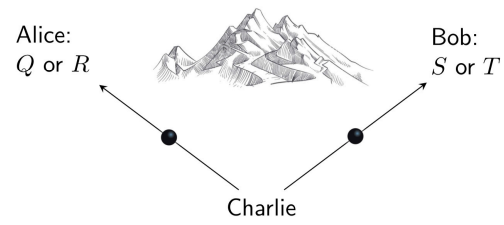
\includegraphics[scale=0.5]{chapters/res/alice-bob-charlie-mountain.png}
    \caption{Charlie prepares two particles, sends one to Alice and one to Bob.}
\end{figure}

By convention binary property values: $Q, R, S, T \in \{\pm 1 \}$. 
Alice decides randomly whether to measure property $Q$ or $R$ and Bob decides randomly to measure 
property $S$ or $T$. \\
Alice and Bob perform their measurement (almost) simultaneously, such that no information about their
result can be transmitted in between. \\ 
After completing this protocol, Alice and Bob need to analyse their measurement data. \\
Consider the quantity:
\begin{equation}
    QS + RS + RT - QT = \underbrace{(Q + R)}_{\pm 2 \text{ or } 0} S + \underbrace{(R - Q)}_{0 \text{ or } \pm 2} T
        = \pm 2
\end{equation}

Denote by $p(q, r, s, t)$ the probability that the system before the measurements is in state 
$Q = q, R = r, S = s, T = t$, then

\begin{align}
    \mathbb{E}[QS + RS + RT - QT] 
        &= \sum_{q, r, s, t \in \{\pm 1 \}} p(\underbrace{qs + rs + rt - qt}_{\pm 2}) \\ 
        %
        &\leq \sum_{q, r, s, t \in \{\pm 1 \}} p(q, r, s, t) \cdot 2 = 2 
\end{align}

By linearity of $\mathbb{E}$, arrive at the following \underline{Bell inequality}:

\begin{equation}
    \mathbb{E}[QS] + \mathbb{E}[RS] + \mathbb{E}[RT] - \mathbb{E}[QT]
        \leq 2
\end{equation}

Each term can be experimentally evaluated, e.g. for $\mathbb{E}[QS]$: \\
Alice and Bob average over cases where Alice measured $Q$ and Bob measured $S$. \\

Compare with "quantum" realization of the experiment: 
Charlie prepares two-qubit singlet state $\statepsi = \frac{1}{\sqrt{2}} (\ket{01} - \ket{10})$
and sends the first qubit to Alice and the second to Bob.
Observables
\begin{align*}
    Q &= \underbrace{Z_1}_{\text{acts on first qubit}}, 
        &&S = \frac{-Z_2 - X_2}{\sqrt{2}} \\
    %
    R &= X_1, &&T = \frac{Z_2 - X_2}{\sqrt{2}}
\end{align*}

Measurement averages (c.f. Exericse 8.1):
\begin{align*}
    \left\langle  QS \right\rangle &= \braketmatrix{\psi}{Q \otimes S}{\psi} = \frac{1}{\sqrt{2}} \\
    \left\langle  RS \right\rangle &= \frac{1}{\sqrt{2}} \\
    \left\langle  RT \right\rangle &= \frac{1}{\sqrt{2}} \\
    \left\langle  QS \right\rangle &= -\frac{1}{\sqrt{2}} 
\end{align*}

\begin{equation*}
    \leadsto  
        \left\langle  QS \right\rangle + 
        \left\langle  RS \right\rangle + 
        \left\langle  RT \right\rangle - 
        \left\langle  QT \right\rangle = 2 \sqrt{2} {\color{red} \nleq 2} \text{ (Violates Bell's inequality!)}
\end{equation*}

Actual labratory experiments (using photons) agree with predictions by quantum mechanics, 
thus not all (implicit) assumptions leading to Bell's inequality can be satisfied: \\

\begin{itemize}
    \item "realism": Physical properties $Q, R, S, T$ have definite values independent of observation
    (measurement).
    \item locality: Alice performing her measurement cannot influence Bob's measurement and vice versa
\end{itemize}

$\leadsto$  Nature is not "\textit{locally realistic}". 
(Most common viewpoint: Realism does not hold)

Practical lesson: Use entanglement as a resource.